\documentclass[../main.tex]{subfiles}

\begin{document}
In questa sezione si analizzano alcune delle librerie scelte per la sperimentazione del paradigma FRP in Scala. Aspetti cruciali dell'analisi delle librerie sono la correttezza rispetto la definizione del paradigma FRP (discussa nel capitolo 2), lo stato attuale della libreria (active, maintenance o EOL) ed il supporto a Scala. La sperimentazione è stata effettuata sviluppando gli stessi esempi con le diverse librerie in analisi: \textit{Sodium}, \textit{Reactify}. Gli esempi sviluppati sono i seguenti:
\begin{itemize}
    \item Sensore di temperatura (\textit{XThermalManagerExample}): flusso di rilevamenti simulati di sensori di temperatura e lavorazioni sui valori per estrarre altri valori come temperatura media e spikes.
    \begin{figure}[H]
        \centering
        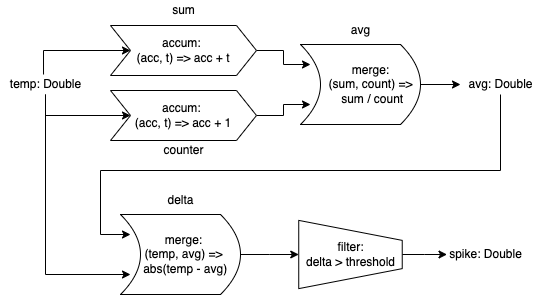
\includegraphics[width=0.9\textwidth]{img/frp-scala-Page-3.drawio.png}
        \caption{Grafo delle dipendenze: temperatura media e spikes}
    \end{figure}
    \item Contatore/ticker (\textit{XTimeFlowExample}): flusso di cambiamenti al valore del contatore, al quale è associata come reazione il calcolo dei millisecondi trascorsi e la stampa del valore.
    \begin{figure}[H]
        \centering
        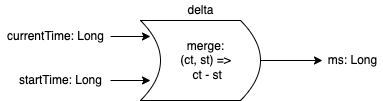
\includegraphics[width=0.7\textwidth]{img/frp-scala-Page-4.drawio.png}
        \caption{Grafo delle dipendenze: timer}
    \end{figure}
\end{itemize}

\section{Sodium}
La libreria open-source Sodium è stata progettata e sviluppata da Stephen Blackheath e Anthony Jones (più altri collaboratori) per fornire una libreria production-ready in diversi linguaggi, tra cui Scala, per promuovere la vera definizione del paradigma FRP e per realizzare un riferimento/benchmark per future librerie.

\begin{table}[H]
\centering
\begin{tabular}{|c|c|}
     \hline
     Repository & https://github.com/SodiumFRP/sodium \\
     \hline
     Versione Latest Release & 1.2.0 \\
     \hline
     Data Latest Release & Ottobre 2019 \\
     \hline
     Data Latest Commit & 3 Febbraio 2020 \\
     \hline
     Supporto Scala & 2.12 \\
     \hline
     Dipendenza Gradle & nz.sodium:sodium:1.2.0 \\
     \hline
\end{tabular}
\caption{Main Info Libreria Sodium}
\end{table}

\section{Reactify}
Reactify è una libreria open-source che permette di sviluppare sistemi col paradigma FRP fornendo un insieme limitato di concetti rispetto ad altre librerie come Sodium. Il programma viene espresso in termini di variabili che cambiano (\textit{Var}) o non cambiano (\textit{Val}) valore nel tempo e nel definire una reazione al cambiamento: tutte le primitive tipiche del paradigma FRP non sono fornite dalla libreria, la quale permette di usare qualsiasi funzionalità di Scala direttamente.

\begin{table}[H]
\centering
\begin{tabular}{|c|c|}
     \hline
     Repository & https://github.com/outr/reactify \\
     \hline
     Versione Latest Release & 4.0.6 \\
     \hline
     Data Latest Release & Maggio 2021 \\
     \hline
     Data Latest Commit & 17 Maggio 2021 \\
     \hline
     Supporto Scala & 2.11, 2.12, 2.13, 3 \\
     \hline
     Dipendenza Gradle & com.outr:reactify\_2.13:4.0.6 \\
     \hline
\end{tabular}
\caption{Main Info Libreria Reactify}
\end{table}

\end{document}

